\documentclass{article}

\usepackage[T2A]{fontenc}
\usepackage[utf8]{luainputenc}
\usepackage[english, russian]{babel}
\usepackage[pdftex]{hyperref}
\usepackage[14pt]{extsizes}
\usepackage{listings}
\usepackage{color}
\usepackage{geometry}
\usepackage{enumitem}
\usepackage{multirow}
\usepackage{graphicx}
\usepackage{indentfirst}
\usepackage[ruled,vlined,linesnumbered]{algorithm2e}

\newenvironment{myalgorithm}[1][htb]
  {\renewcommand{\algorithmcfname}{Алгоритм}
   \begin{algorithm}[#1]%
  }{\end{algorithm}}

\setlength{\parskip}{3mm}
\geometry{a4paper,top=20mm,bottom=20mm,left=25mm,right=15mm}
\setlist{nolistsep, itemsep=0.5cm,parsep=0pt}

\usepackage{xcolor}

\colorlet{mygray}{black!30}
\colorlet{mygreen}{green!60!blue}
\colorlet{mymauve}{red!60!blue}
\colorlet{myred}{red!60!blue}

\lstset{
  backgroundcolor=\color{gray!10},  
  basicstyle=\fontsize{13}{13}\ttfamily,
  columns=fullflexible,
  breakatwhitespace=false,      
  breaklines=true,                
  captionpos=b,                    
  commentstyle=\color{mygreen}, 
  extendedchars=true,              
  frame=single,                   
  keepspaces=true,             
  keywordstyle=\color{blue},      
  language=c++,                 
  numbers=none,                
  numbersep=1pt,                   
  numberstyle=\tiny\color{blue}, 
  rulecolor=\color{mygray},        
  showspaces=false,               
  showtabs=false,                                  
  stringstyle=\color{mymauve},                         
  title=\lstname                
}

\makeatletter
\renewcommand\@biblabel[1]{#1.\hfil}
\makeatother

\begin{document}

\begin{titlepage}

\begin{center}
Министерство науки и высшего образования Российской Федерации \\
\vspace{5mm}
Федеральное государственное автономное образовательное учреждение высшего образования \\
Национальный исследовательский Нижегородский государственный университет им. Н.И. Лобачевского \\
\vspace{1cm}
Институт информационных технологий, математики и механики \\
\vspace{5cm}
\textbf{\large Отчет по лабораторной работе} \\
\vspace{8mm}
\textbf{\Large «Алгоритм Дейкстры»} \\
\end{center}

\vspace{3cm}

\newbox{\lbox}
\savebox{\lbox}{\hbox{text}}
\newlength{\maxl}
\setlength{\maxl}{\wd\lbox}
\hfill\parbox{7cm}{
\hspace*{5cm}\hspace*{-5cm}\textbf{Выполнила:} \\ студентка группы 381706-1 \\ Максимова И. И.\\
\\
\hspace*{5cm}\hspace*{-5cm}\textbf{Проверил:}\\ доцент кафедры МОСТ, \\ кандидат технических наук \\ Сысоев А. В.
}

\vspace{\fill}

\begin{center} 
Нижний Новгород \\ 2020
\end{center}
\end{titlepage}

\setcounter{page}{2}

\tableofcontents

\newpage

\section{Введение}
Задача о кратчайшем пути~--- задача поиска самого короткого пути между двумя вершинами графа, в которой минимизируется сумма весов рёбер, составляющих путь.

\par Значимость данной задачи определяется её различными практическими применениями. Например, в GPS-навигаторах осуществляется поиск кратчайшего пути между точкой отправления и точкой назначения. В качестве вершин выступают перекрёстки, а дороги являются рёбрами, которые лежат между ними. Если сумма длин дорог между перекрёстками минимальна, тогда найденный путь самый короткий.

\par Задача о кратчайшем пути является одной из важнейших классических задач теории графов. Одним из наиболее распространенных алгоритмов ее решения является Алгоритм Дейкстры.

\par В современном мире необходимо иметь возможность быстро принимать решение об изменении маршрута, так, чтобы он всегда оставался оптимальным. Поэтому встает задача об ускорении алгоритма Дейксты, путем распараллеливания вычислений.

\par В настоящий момент, одними из самых популярных API для реализации многопоточности являются: Intel Threading Building Blocs, OpenMP или std::thread. Однако нет универсального ответа на вопрос каким же API лучше всего пользоваться. Поэтому в данной работе я постараюсь определить лучший API для задачи распараллеливания алгоритма Дейкстры.

\par Цель работы~--- разработать параллельный вариант алгоритма Дейкстры и определить каким прикладным программным интерфейсом  лучше воспользоваться для реализации многопоточности.

\newpage

\section{Постановка задачи}
Формулировка задачи: 
\par Дан взвешенный неориентированный граф \verb|G(V,E)| без дуг отрицательного веса. Найти кратчайшие пути от некоторой вершины \verb|a| графа \verb|G| до всех остальных вершин этого графа.

\par Для успешного выполнения данной работы необходимо дополнительно выполнить следующие подзадачи:
 
\begin{enumerate}
\item Изучить и реализовать последовательный алгоритм Дейкстры.
\item Разработать и реализовать параллельный алгоритм Дейкстры с использованием технологий OpenMP, TBB и std::threads.
\item Реализовать набор автоматических тестов с использованием Google C++ Testing Framework для каждой из технологий.
\item Провести расчет ускорения программы для каждой из технологий и определить лучшую. 
\end{enumerate}

\newpage

\section{Метод решения}
Идея алгоритма Дейкстры: 

\par В процессе работы алгоритма поддерживается множество \verb|S| $\subseteq$ \verb|V|, состоящее из вершин \verb|v|, для которых кратчайший путь \verb|dist[a,v]| уже найден. На кадом шаге, алгоритм выбирает одну новую вершину \verb|u| $\in$ \verb|V\S| с наименьшим весом ребра \verb|w(u,v)|, добавляет \verb|u| ко множеству \verb|S| и производит релаксацию ребер, выходящих из \verb|u|, и входящих в вершины, которые еще не принадлежат \verb|S|. Цикл повторяется, пока все вершины не войдут в \verb|S|.

\par Рассмотрим наивную реализацию алгоритма.

\par Каждой вершине из \verb|V| сопоставим метку — минимальное известное расстояние от этой вершины до вершины-источника \verb|a|. На каждом шаге алгоритм посещает новую вершину и пытается уменьшать метки. Работа алгоритма завершается, когда все вершины посещены.

\begin{myalgorithm}[H]
\SetAlgoLined
\SetKwInOut{Input}{Вход}
\SetKwInOut{Output}{Выход}
\SetKwInOut{Data}{Данные}
\Input{граф $G(V,E)$; веса ребер $w(e)\geq 0, e \in E$; вершина-источник $a$}
\Output{расстояние $dist[v]$ от $a$ до каждой вершины $v \in V$; в начале $dist[v] = \infty$, для каждой $v \in V$ }
\Data{массив меток $mark[]$, $mark[v] = true $ - вершина $v$ посещена; в начале $mark[v] = false$, для каждой $v \in V$}
\BlankLine
\BlankLine
$dist[a] = 0$\;
$mark[a] = true$\;
\BlankLine
\For {$v \in V$} {
 $u = Min(dist[]): mark[u] == false$\;
 $mark[u] = true$\;
 \BlankLine
 \ForAll {вершин $k$, смежных с $u$} {
 	\If {$mark[k] == false\ \&\ dist[k] > dist[u] + w(u, k)$} {
  	$dist[k] = dist[u] + w(u, k)$\;
  } } }
\caption{Наивная реализация алгоритма Дейкстры}
\end{myalgorithm}

\newpage

\section{Схема распараллеливания}
Рассмотрим наивную реализацию алгоритм Дейкстры с точки зрения задачи параллелизации вычислений.

\par При параллелизации наивного алгоритма Дейкстры, надо учитывать, что внутри внешнего цикла (стр. 7, алг. 1) необходимо распараллелить поиск минимума в массиве \verb|dist| (стр. 8), и цикл по всем вершинам в стр.10. Причем, чтобы не нарушать логику работы программы, нужно синхронизировать потоки перед записью в глобальные переменную \verb|u|, и добавить барьер перед циклом в стр. 10.

\par Схема распараллеливания наивного алгоритма Дейкстры 1 выглядит следующим образом:    

\begin{myalgorithm}[H]
\SetAlgoLined
\BlankLine
$dist[a] = 0$\;
$mark[a] = true$\;
\BlankLine
\For {$v \in V$} {
 \textcolor{myred}{$u$ =} \textcolor{mygreen}{$Min(dist[]): mark[u] == false$\;}
 \textcolor{mygreen} {$mark[u] = true$\;}
 \textcolor{myred}{$Barrier$\;}
 \textcolor{mygreen} {
 \ForAll {вершин $k$, смежных с $u$} {
 	\If {$mark[k] == false\ \&\ dist[k] > dist[u] + w(u, k)$} {
  	$dist[k] = dist[u] + w(u, k)$\;
  } } }
  }
\caption{Распараллеливания алгоритма Дейкстры 1}
\end{myalgorithm}

\par Черный код - последовательное выполнение, зеленый - зона параллельных вычислений, красный - точка синхронизации потоков. 

\par Наличие барьера в параллельной программе приводит к возникновению дополнительных накладных расходов и простаиванию потоков. Чтобы этого избежать можно модифицировать алгоритм Дейкстры так, что в итоге останется также одна точка синхронизации, но барьер уже не понадобиться. Для этого нужно избавиться от цикла в строке 8. Как мы видим этот цикл возникает в результате поиска минимальной вершины. Поэтому можно воспользоваться знанием структур данных, и модифицировать наивный Алгоритм Дейкстры. Контейнер, в котором поиск минимального элемента может осуществляется за \verb|O(logn)| - приоритетная очередь. 
\par Псевдокод алгоритма Дейкстры с приоритетной очередью: 

\begin{myalgorithm}[H]
\SetAlgoLined
\SetKwInOut{Input}{Вход}
\SetKwInOut{Output}{Выход}
\SetKwInOut{Data}{Данные}
\Input{граф $G(V,E)$; веса ребер $w(e)\geq 0, e \in E$; вершина-источник $a$}
\Output{расстояние $dist[v]$ от $a$ до каждой веришны $v \in V$, В начале $dist[v] = \infty$, для каждой $v \in V$}
\Data{Приоритетная очередь $Queue$, элементами которой являются пары: ключ - $dist[v]$, значение - $v$, где $v \in V $ }
\BlankLine
$Queue = new\ priority\ queue$\;
$dist[a] = 0$\;
$Queue.push(0, a)$\;
\While{Queue not empty} {
$u, dist_u = ExtractMin(Queue)$\;
\If {$dist_u > dist[u]$}{continue\;}
\BlankLine
\ForAll { $v \in V $} {
\If {$dist[v] > dist[u] + w(u, v)$} {
 $dist[v] = dist[u] + w(u, v)$\;
 $Queue.push(dist[v], v)$\; } } }
\caption{Алгоритм Дейкстры с приоритетной очередью}
\end{myalgorithm}

\par Теперь для распараллеливания программы, нужно установить лишь одну точку синхронизации~--- при записи в очередь \verb|Queue| в стр. 12, алг. 3. Это необходимо для обеспечения потокобезопасности. Очередь \verb|Queue| является глобальной по отношению к потокам.

\par Параллелизация внешнего цикла в стр. 4, алг. 3 невозможна, поскольку иначе будет нарушена логика работы программы. Единственным местом для организации параллельных вычислений остается цикл по всем вершинам в стр. 9, алг. 3. Но как нетрудно заметить, этот цикл и является главной вычислительной нагрузкой всего алгоритма.
 
\par Таким образом, схема распараллеливания алгоритма Дейкстры с использование приоритетной очереди выглядит следующим образом: \\   

\begin{myalgorithm}[H]
\SetAlgoLined
\BlankLine
$Queue = new\ priority\ queue$\;
$dist[a] = 0$\;
$Queue.push(0, a)$\;
\While{Queue not empty} {
$u, dist_u = ExtractMin(Queue)$\;
\If {$dist_u > dist[u]$}{continue\;}
\textcolor{mygreen}{
\BlankLine
\ForAll { $v \in V $} {
\If {$dist[v] > dist[u] + w(u, v)$} {
 $dist[v] = dist[u] + w(u, v)$\;
 \textcolor{myred}{$Queue.push(dist[v], v)$\;} } }
 } 
}
\caption{Распараллеливание алгоритма Дейкстры 3}
\end{myalgorithm}

\par Черный код - последовательное выполнение, зеленый - зона параллельных вычислений, красный - точка синхронизации потоков. 

\newpage

\section{Описание программной реализации}
Прежде чем приступать к описанию реализации самого алгоритма Дейкстры, хотелось бы уточнить в каком формате представлен исходный граф.

\par В программе граф представлен матрицей смежности, в которой на пересечении i-й строки  и j-го столбца стоит значение весовой функции соответствующего ребра. Все веса имеют тип \verb|int|. Если ребра \verb|(i,j)| нет, то в данной ячейке таблицы устанавливается значение \verb|INT8_MAX|. Это значение интерпретируется в программе как бесконечность. Матрица смежности храниться в виде вектора:

\vspace{10pt}
\begin{lstlisting}
    std::vector<int> linkedList
\end{lstlisting}
\vspace{-25pt}

\par Для организации работы с графом был реализован тривиальный класс \verb|Graph|, содержащий методы работы с матрицей смежности. Помимо вектора \verb|linkedList| полями класса являются число вершин \verb|V| и ребер \verb|E| графа \verb|G(V,E)|: 

\vspace{10pt}
\begin{lstlisting}
    int numVertex // numVertex = |V|
    int numEdges  // numEdges = |E|
\end{lstlisting}
\vspace{-25pt}

\par Методы данного класса тривиальны и в подробном описании не нуждаются. Отметим только метод \verb|createRandGraph|, который генерирует рандомный граф. Внутри него, происходит инициализация случайных ребер рандомными значениями, с помощью генератора псевдослучайных чисел \verb|std::mt19937|. Ниже перечисленны все методы класса \verb|Graph|:

\vspace{10pt} 
\begin{lstlisting}
    explicit Graph(int _numVertex, int _numEdges);
    void createRandGraph();
    void putEdge(int a, int b, int weightEdge);
    int getNumEdges() const { return numEdges; }
    int getNumVertex() const { return numVertex; }
    const int& operator[](const int i) const { return linkedList[i]; }
\end{lstlisting}
\vspace{-25pt}

\par Вернемся к реализации алгоритма Дейкстры. Алгоритм был достаточно подробно разобран в псевдокоде алгоритма 3. С точки зрения его реализации опишем лишь в каком виде данные хранятся в приоритетной очереди \verb|Queue|.

\par В стандартной библиотеке C++ контейнер \verb|std::priority_queue| хранит элементы в порядке убывания, а в алгоритме Дейкстры нужно получить минимальный элемент из очереди. Чтобы обеспечить быстрый поиск минимального элемента, в программе все значения ключей \verb|dist[v]|, при помещении и изъятии из очереди \verb|Queue| умножаются на \verb|-1|. 

\par Поскольку в данной работе рассмотриваются 3 технологии параллельного программирования: OpenMP, TBB и std::threads, то в следующих подразделах опишем используемые методы API для кажой из технологий.

\par Заметим, что принцип распараллеливания везде и тот же, меняются лишь инструменты параллелизации.

\subsection{OpenMP}
Определения именованных констант, прототипов функций и типов данных OpenMP содержится в файле \verb|omp.h|. 
\par Для параллелизации зеленого цикла в алгориме 4 используется директива \verb|#pragma omp parallel for|. 
\par Запись данных в глобальную очередь \verb|Queue| организована в виде критической секции. Определение критической секции в OpenMP осуществляется при помощи директивы \verb|#pragma omp critical|.
\par Псевдокод параллельного фрагмента алгоритма Дейкстры с использованием OpenMP:

\vspace{10pt}
\begin{lstlisting}
    #pragma omp parallel for
      for (int v = 0; v < numVertex; ++v)
        if (dist[v] > dist[u] + w[u, w])
          dist[v] = dist[u] + w[u, w]
    #pragma omp critical
	  Queue.push(dist[v], v)
\end{lstlisting}
\vspace{-25pt}

\subsection{TBB}
Для параллелизации зеленого цикла в алгоритме 4 используется функция
\verb|tbb::parallel_for|, объявленная в заголовочном файле \verb|tbb/tbb.h|. В качестве параметров эта функция принимает:

\begin{enumerate}
\item Одномерное итерационное пространство \verb|tbb::blocked_range| ~--- рекурсивно делимый полуинтервал \verb|[0; N)|, где \verb|N| - число вершин графа. Значение параметра размера порции вычислений \verb|grainsize| явно не устанавливается, поскольку разделение на порции осуществляется планировщиком TBB автоматически.

\item Лямбда, реализующая вычисления тела цикла. А именно, она совершает релаксацию значений текущих расстояний от вершин \verb|v|, попавших в отведенное лямбде итерационное пространство, до вершины-источника \verb|a|.
\end{enumerate}

\par Для обеспечения записи в глобальную очередь используется потокобезопасная реализация очереди \verb|tbb::concurrent_queue|. В библиотеке TBB реализован собственный планировщик задач, работающй гораздо эффективнее на ориентированных под него структурах данных. Несколько потоков могут одновременно записывать и извлекать элементы из такой очереди. Очередь не имеет операций блокировки. Поэтому в реализации алгоритма Дейкстры с использованием TBB явная  синхронизация не нужна.

\par Псевдокод параллельного фрагмента алгоритма Дейкстры с использованием TBB:

\vspace{10pt}
\begin{lstlisting}
    tbb::concurrent_queue Queue
    ...
    tbb::parallel_for(
        tbb::blocked_range<int>(0, numVertex),
        [&](const tbb::blocked_range<int>& r) {
          for (int v = r.begin(); v != r.end(); ++v)
            if (dist[v] > dist[u] + w[u, w])
              dist[v] = dist[u] + w[u, w]
              Queue.push(dist[v], v);
        })
\end{lstlisting}
\vspace{-25pt}

\subsection{std::threads}
Праллелизация программы с использованием API \verb|std::thread| осуществляется путем создания объектов \verb|std::thread|. Под каждый поток нужен свой объект класса. В данной работе реализован статический массив \verb|th_array| объектов \verb|std::thread|, размером \verb|count_th|.

\par Заранее необходимо вычислить объем порции данных \verb|dose|, обрабатываемых каждым потоком. Это делается путём взятия целой части от деления общего количества вершин графа на количество потоков. Остаток от деления \verb|rem| добавляется к порции последнего потока. 

\par Для паралллелизации зеленого цикла алгоритма 4, нужно в цикле по числу потоков \verb|count_th|, проинициализировать каждый поток ламбдой. Сразу после инициализации поток переходит в состояние исполнения. 

\par В лямбду передается номер потока, на котором она будет исполняться и размер порции вычислений для данного потока. Поскольку гарантированный размер порций вычислений у каждого потока одинаков и равен \verb|dose|, то в лямбду потока \verb|th_array[i]| передается только остаток от деления \verb|remainder[i]|, где \verb|remainder[i]| = 0, для всех всех потоков, кроме последнего. Для последнего потока  
\verb|remainder[count_th-1]| равен остатку \verb|rem|.

\par Сама лямбда совершает релаксацию значений текущих расстояний от вершин v, попавших в отведенное лямбде итерационное пространство, до вершины-источника \verb|a|.

\par Для синхронизации потоков при записи данных в очередь \verb|Queue| используется примитива синхронизации \verb|std::mutex|. Над мьютексом используется обертка \verb|std::lock_guard|, которая предоставляет удобный механизм в стиле RAII для владения мьютексом на время блока с областью видимости.

\par После запуска потоков, дожидаемся их завершения, выполняя операцию блокировки главного потока \verb|std::thread::join|

\par Псевдокод параллельного фрагмента алгоритма Дейкстры с использованием std::threads:

\vspace{10pt}
\begin{lstlisting}
    std::mutex mtx
    std::thread th_array[count_th]
    int dose = count vertex / count_th
    int rem = count vertex % count_th
    int remainder[count_th] = {0}
    remainder[count_th - 1] += rem
    ...
    for (int i = 0; i < count_th; ++i)
      th_array[i] = std::thread([&](int num_th, int remnd) {
          for (int v = num_th * dose; v < (num_th + 1) * dose + remnd; ++v)
            if (dist[v] > dist[u] + w[u, w])
              dist[v] = dist[u] + w[u, w]
              std::lock_guard<std::mutex> locker(mtx)
              Queue.push(dist[v], v)
      }, i, remainder[i])
          
    for (int i = 0; i < count_th; ++i) th_array[i].join()
\end{lstlisting}
\vspace{-25pt}

\newpage

\section{Подтверждение корректности}
Для отслеживания корректности выполнения программы для каждой из технологий был реализован набор тестов, разработанных с помощью Google C++ Testing Framework.

\par Тесты, проверяющие корректность создания графа:

\begin{itemize}
\item \verb|Test_Constructor_Graph_Error_Zero_Vertex|~--- проверка на создание непустого графа;
\item \verb|Test_Constructor_Graph_Error_Negative_Vertex|~--- проверка на неотрицательность числа вершин графа;
\item \verb|Test_Constructor_Graph_Error_Too_Many_Edges|~--- проверка на количество ребер в графе. Число ребер в графе не должно превышать числа ребер в полном графе \verb|n*(n-1)/2|, где n - число вершин.
\item \verb|Test_Can_Create_Random_Graph|~--- проверка на способность инициализировать граф случайными ребрами
\item \verb|Test_Can_Create_Random_Graph_Min_Edges|~--- проверка на способность инициализировать дерево случайными ребрами
\item \verb|Test_Can_Create_Random_Graph_Max_Edges|~--- проверка на способность инициализировать полный граф случайными ребрами
\end{itemize}
\par Тесты, проверяющие работоспособность алгорима Дейкстры:
\begin{itemize}
\item \verb|Test_No_Throw_Execute_Dijkstra_Alg|~--- способность выполнить алгоритм без возникновения исключений;
\item \verb|Test_Right_Execute_Dijkstra_Alg_Linked_Graph|~--- способность верно выполнить алгоритм на связаном графе;
\item \verb|Test_Execute_Dijkstra_Alg_Unlinked_Graph|~--- способность верно выполнить алгоритм на связаном графе;
\end{itemize}

\par Набор данных тестов был доведен до успешного выполнения для каждой из технологий параллельного программирования.

\newpage

\section{Результаты экспериментов}
Вычислительные эксперименты для оценки эффективности параллельного варианта Алгоритма Дейкстры проводились на ПК со следующими параметрами:

\begin{itemize}
\item ОС: Microsoft Windows 10 Home;
\item Процессор: Intel(R) Core(TM) i5-7200U @ 2.50GHz;
\item Тактовая частота процессора: 2.7 GHz;
\item Число ядер: 2;
\item Оперативная память: 4 GБ, 2400 MHz;
\item Размер кэша L1, L2, L3: 128, 512, 3072 KB;
\end{itemize}

\par В экспериментах осуществлялся замер времени выполнения алгоритма Дейкстры 3 и высчитывалось ускорение программы путем деления времени исполнения последовательного алгоритма на время параллельного. 

\par Для проведения экспериментов задействовано 4 потока. Переменным параметром является число вершин \verb|n| в графе. Числе ребер берется равным \verb|n*(n-1)/10|. Результаты экспериментов представлены на рис. 1.

\begin{figure}[h]
\centering
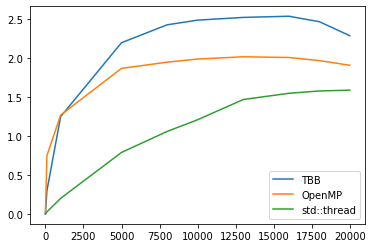
\includegraphics[scale=1.1]{../../../../modules/reports/maximova_i_dijkstra_algorithm/speedup.png}
\caption{Ускорение программы}
\end{figure}

\newpage

\par Чтобы грамотно оценивать свои результаты вспомним немного теорию. 

\par Закон Амдала гласит: 

\begin{equation}
Speedup \leq \frac{1}{(1-pctPar) + \frac{pctPar}{p}}
\end{equation} 

где \verb|pctPar|~--- процент времени выполнения параллельного фрагмента кода, \verb|p|~--- число потоков. 

\par Проведя эксперименты для каждой технологией параллельного программирования, был получен приблизительно одинаковый результат:

\begin{equation}
pctPar(n=1000)\approx 0.85 \Rightarrow Speedup(p = 4) \leq 2.75
\end{equation}

\par Таким образом, максимальное ускорение~--- ускорение в 2.75 раз. Как видно из риc. 1, такого значения мы не достигаем, хотя приближаемся достаточно близко. Достижению максимального ускорения программы препятствуют следующие причины: 

\begin{itemize}
\item Стоимость синхронизации при записи в глобальную очередь.
\item Плохая пространственная локальность. При параллелизации цикла данные из матрицы смежности читаются не последовательно, что приводит к возникновению кеш-промахов и затормаживанию программы.
\end{itemize} 

\par Проанализируем каждый график на рис. 1.

\par Худший результат показала реализация алгоритма Дейкстры с использованием std::thread. Это объясняется тем, что при использовании встроенных потоков для реализации алгоритмов более вероятно возникновение таких ошибок многопоточности, как состязание потоков и взаимная блокировка. TBB и OpenMP разработаны для создания многопоточности с целью обеспечения производительности и масштабируемости, поэтому они и должны были показать лучшую эффективность по отношению к std::thread.

\par TBB или OpenMP создают пул потоков и управляют им: синхронизация и планирование потоков выполняются автоматически.
 
\par Тем не менее вторую ступень пьедестала занимает OpenMP. Ускорение программы с использованием OpenMP не так велико, по отношению к TBB, поскольку программу тормозит принудительная синхронизация потоков при записи в \verb|std::priority_queue|.

\par Лучшей оказалась реализация алгоритма с использованием TBB. В отличии от OpenMP в TBB реализованы потокобезопасные контейнеры, в частности \verb|tbb::concurrent_queue|, которые перекладывают всю ответственность на планировщик задач TBB. С помощью метода захвата задач в сочетании с алгоритмом динамического балансирования нагрузки, предоставляемого планировщиком задач, TBB позволяет загружать все процессорные ядра полезной нагрузкой. В итоге накладных
расходов при работе с потокобезопасными контейнерами в параллельных приложениях меньше, чем при использовании стандартных контейнеров STL.

\par Обратим внимание на то, что не всегда TBB, лучше чем OpenMP. На рисунке 1 видно, что при малом числе вершин ($n < $ 1000) TBB оказывается менее эффективен, по сравнению с OpenMP. Это связано, с тем, что для обслуживания \verb|tbb::concurrent_queue| требуется больше накладных расходов, чем для очереди STL. Для статического планирования (OpenMP), накладные расходы минимальны. Тем не менее динамическое планирование (TBB) имеет некоторые накладные расходы, но это не имеет значения, если рабочая нагрузка достаточна. 
 
\par Также заметим, что графики, переходя отметку в  $n \approx$ 16000 снижаются. Уменьшение ускорения для более крупных графов связано с тем, что данные в программу подаются быстрее, чем успевают обрабатываться. Пропускная способность системной шины снижается. 
\par В итоге, лучшей технологией для реализации параллельного алгоритма Дейкстры на приоритетной очереди оказалась TBB.

\newpage

\section{Заключение}
Подведем результаты выполнения задач, поставленных в разделе 2.

\par В ходе выполнения данной работы был подробно изучен алгоритм Дейкстры поиска кратчайших маршрутов на графе. 

\par Реализован последовательный алгоритм в двух модификациях: наивный алгоритм и алгоритм с использованием приоритетной очереди. В процессе работы было установлено, что для реализации параллельного алгоритма Дейкстры лучше воспользоваться приоритетной очередью.

\par Успешно выполнена основная задача работы: разработка и реализация эффективной параллельной версии алгоритма Дейкстры с использованием технологий: OpenMP, TBB, std::threads.

\par Разработаны и доведены до успешного выполнения тесты, созданные с использованием Google C++ Testing Framework.

\par В конце были проведены эксперименты, по результатам которых  лучшей технологией для реализации параллельного алгоритма Дейкстры оказалась библиотека TBB. Все результаты проанализированы и задокументированы в разделе 7.

\newpage

\section{Список литературы}
\begin{enumerate}
\bibitem{OMP} Гергель В.П. Учебный курс «Введение в методы параллельного программирования», раздел «Параллельное программирование с использованием OpenMP». Нижний Новгород, ННГУ, 2007, 33 с.

\bibitem{TBB} А.А. Сиднев, А.В. Сысоев, И.Б. Мееров. Учебный курс «Технологии разработки параллельных программ», раздел «Создание параллельной программы», «Библиотека Intel Threading Building Blocks~--- краткое описание». Нижний Новгород, ННГУ, 2007, 29 с. 

\bibitem{STD} Справочник по конструкциям языка C++, раздел std::thread // URL: https://ru.cppreference.com/

\bibitem{Parallel Technologies} Michael J Voss. "Intel Threading Building Blocks, OpenMP, or native threads?". Intel Corpotation, Development Topics \& Technologies, 2011. // URL: \linebreak https://software.intel.com/content/www/us/en/develop/articles/intel-threading-building-blocks-openmp-or-native-threads.html

\bibitem{Speedup} Levent A., Clay B., Martyn C., et.al. "Intel Guide for Developing Multithreaded Applications". Intel Corpotation, Development Topics \& Technologies, 2012, 133 p. // URL: http://www.intel.com/software/threading-guide
\end{enumerate}

\newpage

\section{Приложение}
\subsection{Последовательный алгоритм Дейкстры}
\lstinputlisting[language=C++]{../../../../modules/task_1/maximova_i_dijkstra_algorithm/dijkstra_algorithm.h}
\lstinputlisting[language=C++]{../../../../modules/task_1/maximova_i_dijkstra_algorithm/dijkstra_algorithm.cpp}
\lstinputlisting[language=C++]{../../../../modules/task_1/maximova_i_dijkstra_algorithm/main.cpp}

\subsection{OpenMP}
\lstinputlisting[language=C++]{../../../../modules/task_2/maximova_i_dijkstra_algorithm/dijkstra_algorithm.h}
\lstinputlisting[language=C++]{../../../../modules/task_2/maximova_i_dijkstra_algorithm/dijkstra_algorithm.cpp}
\lstinputlisting[language=C++]{../../../../modules/task_2/maximova_i_dijkstra_algorithm/main.cpp}

\subsection{TBB}
\lstinputlisting[language=C++]{../../../../modules/task_3/maximova_i_dijkstra_algorithm/dijkstra_algorithm.h}
\lstinputlisting[language=C++]{../../../../modules/task_3/maximova_i_dijkstra_algorithm/dijkstra_algorithm.cpp}
\lstinputlisting[language=C++]{../../../../modules/task_3/maximova_i_dijkstra_algorithm/main.cpp}

\subsection{std::threads}
\lstinputlisting[language=C++]{../../../../modules/task_4/maximova_i_dijkstra_algorithm/dijkstra_algorithm.h}
\lstinputlisting[language=C++]{../../../../modules/task_4/maximova_i_dijkstra_algorithm/dijkstra_algorithm.cpp}
\lstinputlisting[language=C++]{../../../../modules/task_4/maximova_i_dijkstra_algorithm/main.cpp}


\end{document}
